% Adjust these for the path of the theme and its graphics, relative to this file
%\usepackage{beamerthemeFalmouthGamesAcademy}
\usepackage{../../beamerthemeFalmouthGamesAcademy}
\usepackage{multimedia}
\graphicspath{ {../../} }

% Default language for code listings
\lstset{language=C++,
        morekeywords={each,in,nullptr}
}

% For strikethrough effect
\usepackage[normalem]{ulem}
\usepackage{wasysym}

\usepackage{pdfpages}

% http://www.texample.net/tikz/examples/state-machine/
\usetikzlibrary{arrows,automata}

\begin{document}
\title{Twitter bots}
\subtitle{COMP140: Creative Computing --- Hacking}

\frame{\titlepage} 

\begin{frame}{Today's class}
    \begin{itemize}
        \item RESTful web APIs
        \item Tutorial / live coding: a simple Twitter bot in Python
        \item OAuth
        \item API hacking: sprint review and general support
        \item At 5pm in the Chapel: guest lecture by Barry Caudill, Firaxis Games
    \end{itemize}
\end{frame}

\part{The Twitter API}
\frame{\partpage}

\begin{frame}{REST}
    \begin{itemize}
        \item REST = \textbf{Representational State Transfer} \pause
        \item Many web services provide a \textbf{REST API} \pause
            \begin{itemize}
                \item Including your COMP110 client/server coding task! \pause
            \end{itemize}
        \item An API is \textbf{RESTful} if it is: \pause
            \begin{itemize}
                \item Based on a \textbf{client-server model}: clients send requests to a server \pause
                \item \textbf{Stateless}: each request from the client is self-contained \pause
                \item \textbf{Cacheable}: the API makes clear which responses can and cannot be cached \pause
                \item \textbf{Layered}: the ``server'' may actually be a cluster of machines \pause
                \item Uses a \textbf{uniform interface}: e.g.\ HTTP requests, URLs, XML, JSON, ...
            \end{itemize}
    \end{itemize}
\end{frame}

\begin{frame}{Twitter API}
    \begin{itemize}
        \item Twitter provides a REST API \pause
        \item Example: to post a tweet \pause
            \begin{itemize}
                \item (see documentation at \url{https://dev.twitter.com/rest/reference/post/statuses/update}) \pause
                \item The client makes an \textbf{HTTP POST request} to
                    \url{https://api.twitter.com/1.1/statuses/update.json?status=Hello+world} \pause
                \item The \textbf{HTTP request header} contains authentication information for the app
                    and for the user \pause
                \item The \textbf{response} from the server is a JSON document containing information about the
                    posted tweet
            \end{itemize}
    \end{itemize}
\end{frame}

\begin{frame}{Libraries}
    \begin{itemize}
        \item Working with REST APIs directly through HTTP requests can be cumbersome \pause
        \item For most popular web services, there are many \textbf{libraries} (official and third party)
            which wrap the REST APIs in a more programmer-friendly interface \pause
        \item For Twitter: \url{https://dev.twitter.com/overview/api/twitter-libraries} \pause
        \item For today's live coding, I will be using the \textbf{Tweepy} library for Python
    \end{itemize}
\end{frame}


\part{Your first Twitter bot}
\frame{\partpage}

\begin{frame}{Account set up}
    \begin{itemize}
        \item Go to \url{https://www.twitter.com} and \textbf{either}
            \begin{itemize}
                \item Create an account, \textbf{or}
                \item Sign in to your existing account
            \end{itemize}
        \item NB: Twitter \textbf{requires} app developers to add a \textbf{mobile phone number} to their accounts
            (don't ask me why...)
    \end{itemize}
\end{frame}

\begin{frame}{Application set up}
    \begin{itemize}
        \item Go to \url{https://apps.twitter.com}
        \item Click on \textbf{Create New App}
        \item Fill in the required details and agree to the license agreement
    \end{itemize}
\end{frame}

\begin{frame}{Project set up}
    \begin{itemize}
        \item Open \textbf{PyCharm} and create a \textbf{new project}
        \item Go to \textbf{File} $\to$ \textbf{Settings} $\to$ \textbf{Project} $\to$ \textbf{Project Interpreter}
        \item Click the $+$ button next to the list of packages
        \item Search for and install the \texttt{tweepy} package
    \end{itemize}
\end{frame}

\begin{frame}[fragile]{Your first bot}
    \begin{itemize}
        \item Enter the following code, but \textbf{don't} run it yet
    \end{itemize}
    \begin{lstlisting}[language=Python]
import tweepy

CONSUMER_KEY = '...'
CONSUMER_SECRET = '...'
ACCESS_KEY = '...'
ACCESS_SECRET = '...'

auth = tweepy.OAuthHandler(CONSUMER_KEY, CONSUMER_SECRET)
auth.set_access_token(ACCESS_KEY, ACCESS_SECRET)

api = tweepy.API(auth)
api.update_status("Hello, world!")
    \end{lstlisting}
\end{frame}

\begin{frame}{Adding your API keys}
    \begin{itemize}
        \item Go to \url{https://apps.twitter.com} and click on your app
        \item Click on \textbf{Keys and Access Tokens}
        \item Copy and paste the \textbf{Consumer Key} and \textbf{Consumer Secret} into the code,
                replacing the \texttt{...}
            \begin{itemize}
                \item Do this \textbf{carefully} -- ensure there are no extraneous spaces or other characters between the \lstinline{'} quotes
            \end{itemize}
        \item Click on \textbf{Create my access token}
        \item Copy and paste the \textbf{Access Token} and \textbf{Access Token Secret} into the code,
            replacing the \texttt{...}
    \end{itemize}
\end{frame}

\begin{frame}{API keys: best practices}
    \begin{itemize}
        \item Many web APIs require an \textbf{API key}
        \item This is like a \textbf{password} and should be kept \textbf{secret}
        \item Code in a world-readable GitHub repository is \textbf{not secret}!
        \item Easy solution: put your API keys in a separate source / header / configuration file,
            and use \texttt{.gitignore} to keep that file out of the repository
                \begin{itemize}
                    \item NB: For assignment submissions via LearningSpace,
                        please \textbf{do} include your API keys so that we can test your code!
                \end{itemize}
        \item Other solutions:
            \url{http://programmers.stackexchange.com/q/205606}
    \end{itemize}
\end{frame}

\begin{frame}{Fin}
    \begin{itemize}
        \item Run the code
        \item Open the twitter app or website and admire your bot's first tweet!
        \item You now know how to tweet any text string --- integrate this into your Python code as you see fit
        \item Refer to the docs on \url{http://www.tweepy.org}
            for how to do more interesting things, e.g.\ reading and replying to other people's tweets
    \end{itemize}
\end{frame}

\begin{frame}{Further reading}
    \begin{itemize}
        \item Twitter, ``Automation rules and best practices''.
            \url{https://support.twitter.com/articles/76915}
        \item Darius Kazemi, ``Basic Twitter bot etiquette''.
            \url{http://tinysubversions.com/2013/03/basic-twitter-bot-etiquette/}
    \end{itemize}
\end{frame}



\part{User authentication with OAuth}
\frame{\partpage}

\begin{frame}[fragile]{User authentication}
    \begin{lstlisting}[language=Python]
ACCESS_KEY = '...'
ACCESS_SECRET = '...'

auth = tweepy.OAuthHandler(CONSUMER_KEY, CONSUMER_SECRET)
auth.set_access_token(ACCESS_KEY, ACCESS_SECRET)
    \end{lstlisting}\pause
    \begin{itemize}
        \item OK for creating a bot that only ever tweets on its own account \pause
        \item Not suitable for writing a game component that allows users to use
            their own Twitter accounts, i.e.\ tweets on the user's behalf
    \end{itemize}
\end{frame}

\begin{frame}{OAuth}
    \begin{itemize}
        \item Twitter (and many other web services) use \textbf{OAuth} \pause
        \item Allows you (the user) to use a third-party app without giving it your account password \pause
        \item OAuth is yet another API to get to grips with... \pause
        \item Tweepy has a Twitter-specific wrapper for OAuth
    \end{itemize}
\end{frame}

\begin{frame}[fragile]{Using OAuth}
    \begin{lstlisting}[language=Python]
import tweepy
import webbrowser

CONSUMER_KEY = '...'
CONSUMER_SECRET = '...'

auth = tweepy.OAuthHandler(CONSUMER_KEY, CONSUMER_SECRET)

print "Opening Twitter website -- please log in"
webbrowser.open(auth.get_authorization_url())
verifier = raw_input("Verification code:")
auth.get_access_token(verifier)

api = tweepy.API(auth)
api.update_status("Hello, world!")
    \end{lstlisting}
\end{frame}

\begin{frame}{Staying logged in}
    \begin{itemize}
        \item Store \lstinline{auth.access_token} and \lstinline{auth.access_token_secret} along with your
            application's saved data \pause
        \item Now these can be reloaded and passed to \lstinline{auth.set_access_token},
            just like in our first bot example
    \end{itemize}
\end{frame}


\part{Sprint reviews and general support}
\frame{\partpage}

% -------------------------------------------------------

%\part{The compiler}
%\frame{\partpage}
%
%\begin{frame}
%	\frametitle{The build process}
%	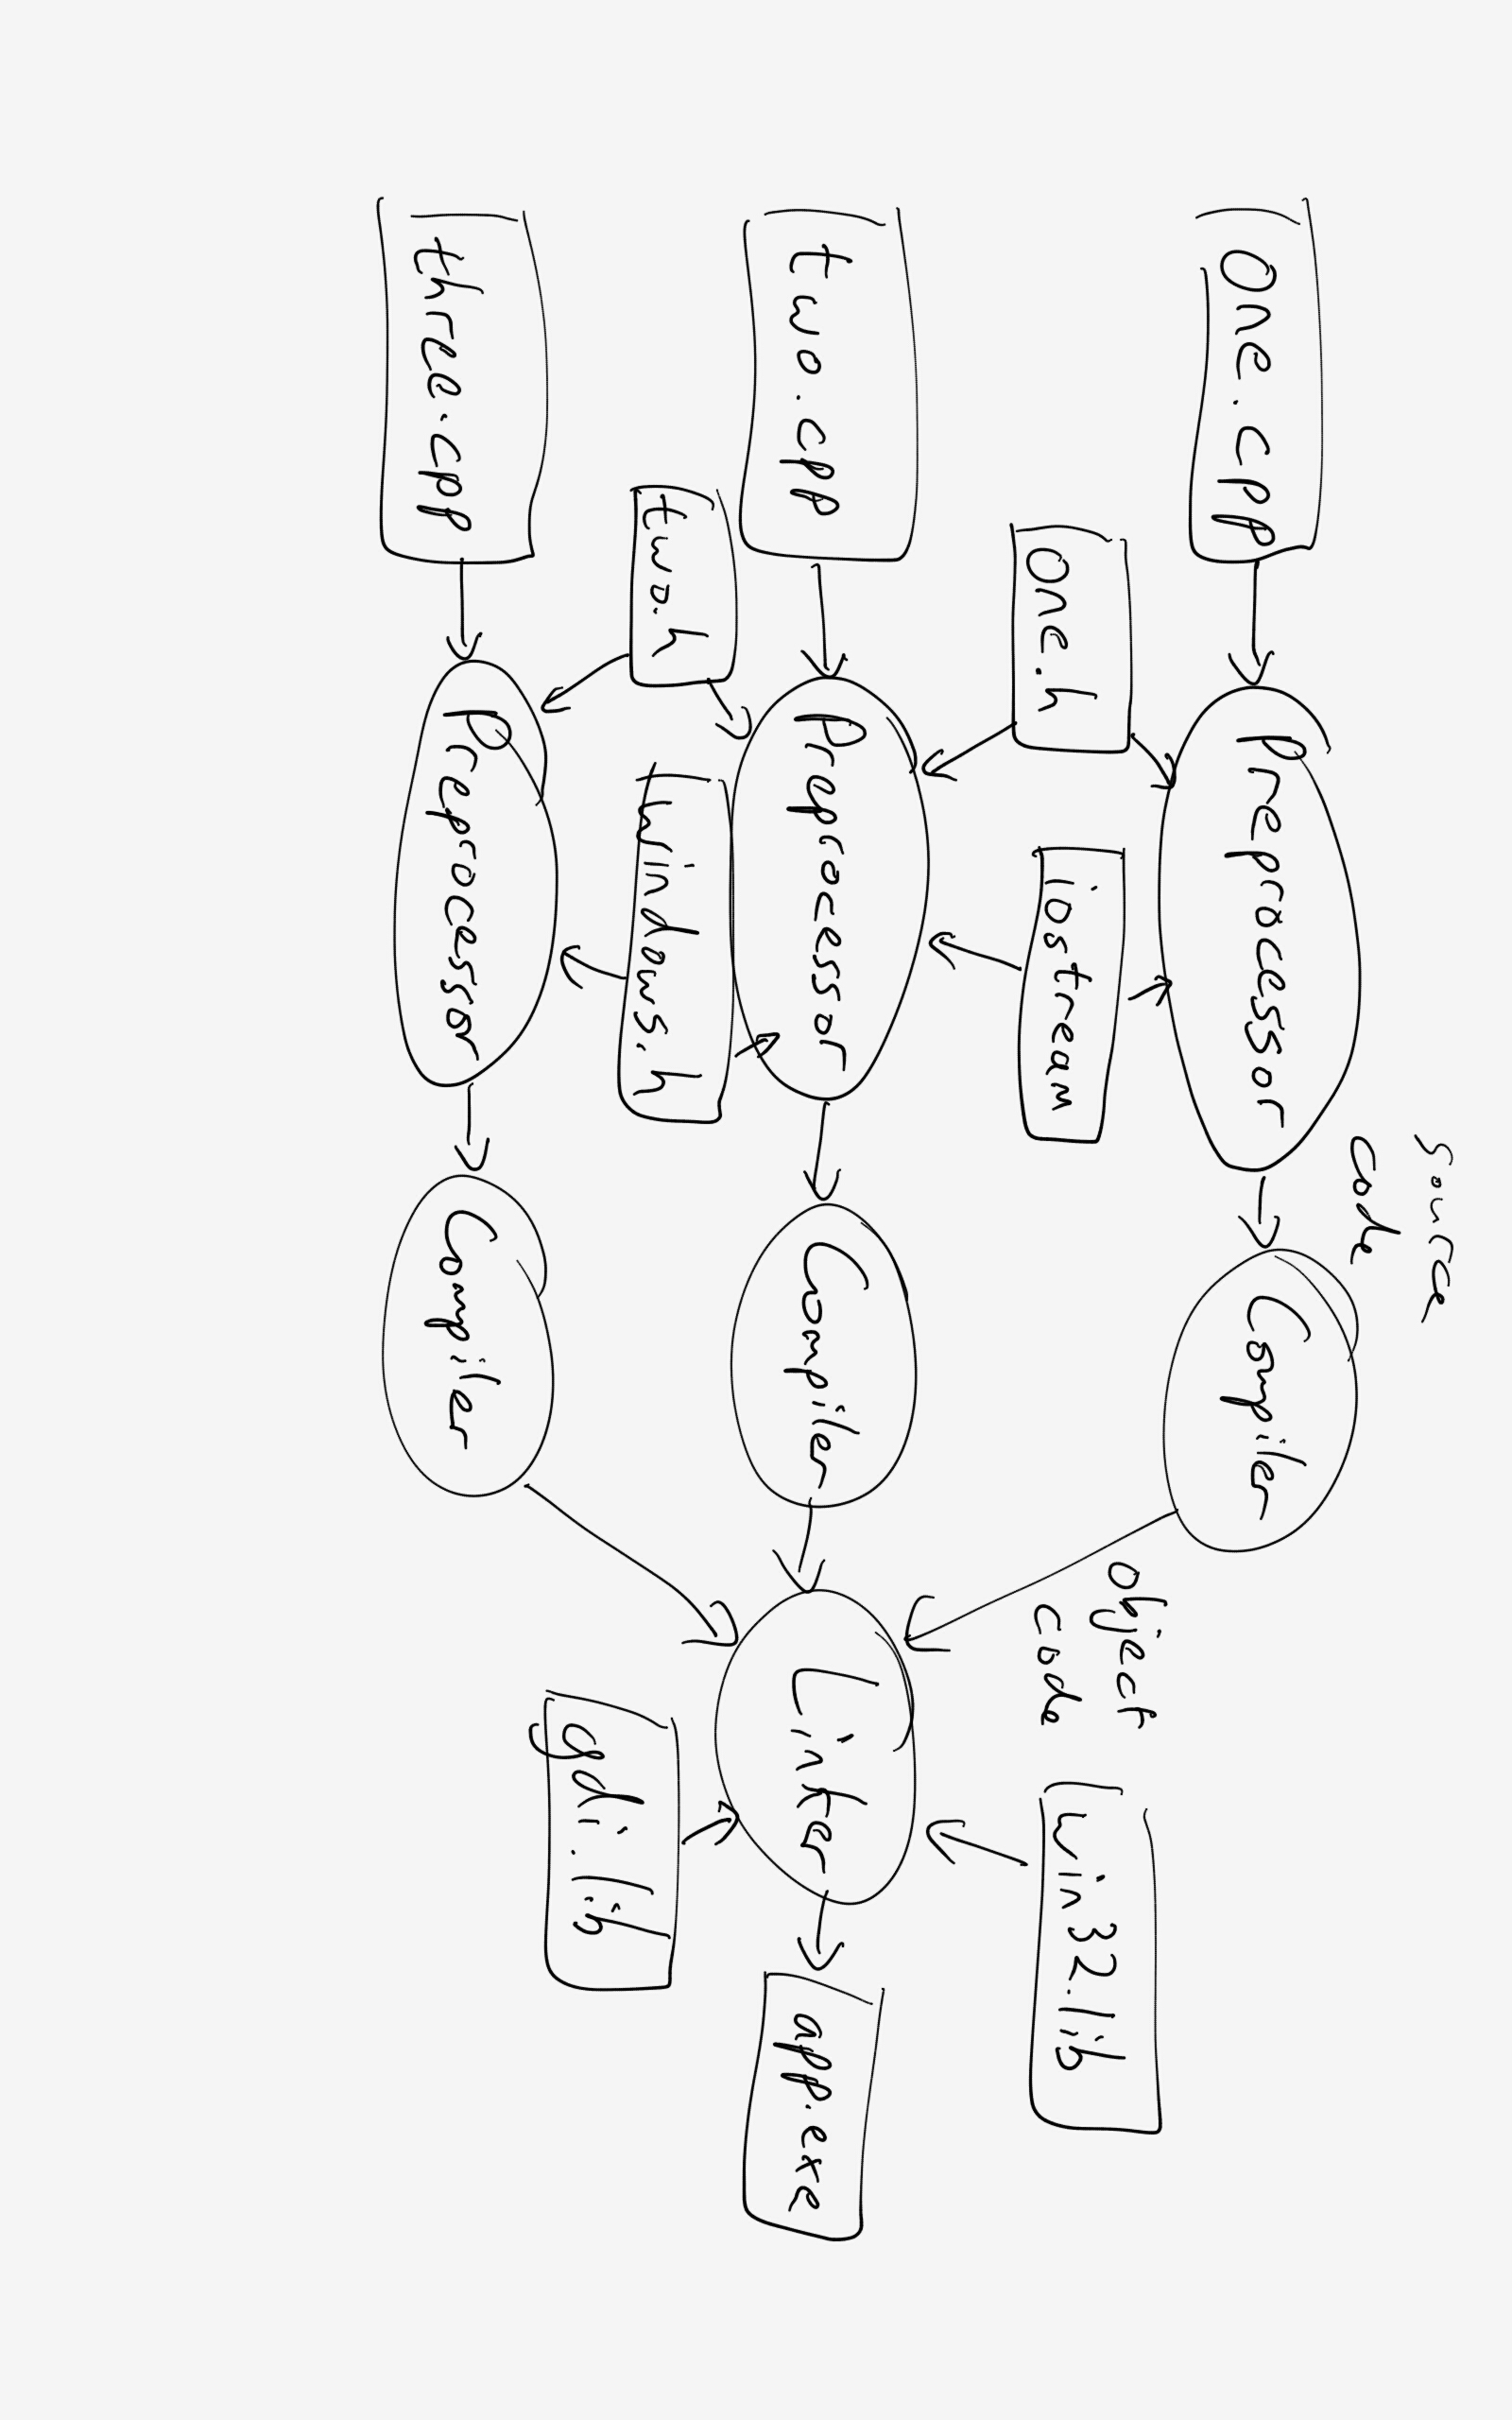
\includegraphics[height=\textwidth,angle=90]{compiler_sketch}
%\end{frame}

\end{document}
